\documentclass[conference]{IEEEtran}
\usepackage{cite}
\usepackage{url}
\usepackage{amsmath,amssymb}
\usepackage{newtxtext,newtxmath}
\usepackage{graphicx}
\usepackage{booktabs}
\usepackage{array}
\def\IEEEkeywordsname{Keywords}
\begin{document}

\title{External Validation of a Seven-Weight Scorecard versus Tree Ensembles in Ovarian Cancer Risk Prediction}

\author{\begin{tabular*}{\textwidth}{@{\extracolsep{\fill}}ccc@{}}
{\bfseries Jiayi Yao} & {\bfseries Zooey Lane Go Hua} & {\bfseries Vritika S Sharma}\\
\textit{BASIS Independent Bellevue} & \textit{Issaquah High School} & \textit{Issaquah High School}\\
Bellevue, WA, USA & Issaquah, WA, USA & Issaquah, WA, USA\\
High School Student & High School Student & High School Student\\
yaojiayi2020@gmail.com & Zooey.hua@gmail.com & vritikas01@gmail.com\\
\end{tabular*}}

\maketitle

\begin{abstract}
Preoperative blood tests help decide whether an ovarian mass requires
cancer surgery; a model that degrades silently at a new hospital can
delay surgery or trigger unnecessary operations. This paper asks whether
more complex machine learning models transfer better to new hospitals
than simple ones. Eight models (a CA125 cutoff rule, the clinical
formulas ROMA and CPH-I, a logistic regression, an integer scorecard,
and three tree ensembles) were trained on a Chinese dataset
(349 patients) and tested, unchanged, on two other Asian cohorts (West
China, 380 patients; Japan, 177). On the 100 West China patients with measured
biomarkers, the scorecard (area under the ROC curve, 0.971) was not
significantly different from the logistic regression (0.941) and ROMA
(0.965), and was numerically the highest. A simulation calibrated to
the real data, intended only as an illustrative counterexample, showed
that under the simulated concept drift examined here the flexible
models' advantage diminished and reversed. Within these small Asian
cohorts, the scorecard performed no worse than far more complex
ensembles and, at its fixed high-risk tier, missed fewer cancers than
the published formulas at their cutpoints; generalization beyond these
cohorts requires larger validation studies.
\end{abstract}

\begin{IEEEkeywords}
ovarian cancer; risk prediction; scorecard; external validation;
transportability
\end{IEEEkeywords}

\section{Introduction}

Ovarian cancer is the most lethal gynecologic cancer, and most cases
are found late. When a pelvic mass is found, whether to send the patient to a
specialist cancer surgeon depends on preoperative risk, and getting it
wrong in either direction is costly. That decision currently relies on two blood proteins, CA125
(cancer antigen 125) and HE4 (human epididymis protein 4), measured
cheaply before surgery and combined either by fixed formulas such as
the Risk of Ovarian Malignancy
Algorithm (ROMA)~\cite{moore2011} and the Copenhagen Index
(CPH-I)~\cite{karlsen2015}, or by a fitted model. Machine learning models have been proposed
for the same task, usually with strong results on the data they were
trained on but little testing at other
hospitals~\cite{kawakami2019,christodoulou2019,wynants2020}.

Lu et al.~\cite{lu2020} trained machine-learning models on the
Changzhou cohort reused here, selecting HE4 and CEA for a decision
tree that outperformed ROMA and logistic regression on a held-out
split. Our work adds a hand-computable scorecard, applies every model
frozen to two Asian cohorts unseen during training, and asks how much
of such an advantage survives the move to a new hospital.

This paper asks two linked questions. First, does model complexity
translate into performance that survives a move to a new hospital?
Second, can a model simple enough to be computed at the bedside (an
integer scorecard) match the more complex alternatives?
Interpretability arguments favor such
simple models in high-stakes medicine~\cite{rudin2019,caruana2015,ustun2016}.
We trained eight models on one Chinese cohort, applied them unchanged
to two independent Asian cohorts, and measured discrimination,
calibration, and decision consequences, plus a simulation of when
complex models help.

\section{Methods}

\subsection{Data}

Three public, anonymized datasets were used
\cite{dataset1,dataset2,machida2023}. Institutional review board approval was not required for
re-analysis of public, de-identified data; the cohorts are a
training cohort from Changzhou,
Jiangsu, China (349 patients; 171 ovarian cancers, 178 benign masses;
Mendeley Data~\cite{dataset1}, \url{doi:10.17632/th7fztbrv9.11}, from
the study by Lu et al.~\cite{lu2020}), a
second Chinese
cohort from the West China Second University Hospital of Sichuan
University, Chengdu (380 patients; 188 cancers, 192 benign cysts;
figshare~\cite{dataset2}, \url{doi:10.6084/m9.figshare.28831256}), and a
Japanese cohort (177 patients; 27
cancers, 150 healthy women; Karger figshare~\cite{machida2023},
\url{doi:10.6084/m9.figshare.24235450}). Each patient has four features:
CA125
(U/mL), HE4 (pmol/L), age, and menopausal status. The source files are
\texttt{chinese training dataset(All Raw Data).csv},
\texttt{west\_china.xlsx}, and \texttt{japanese.xlsx};
\texttt{src/clean\_data.py} harmonizes them into the three processed
files used by every analysis. In the training cohort,
scattered missing biomarker values were filled by each feature's
cohort median. Externally, HE4 was not measured for 74\% of West China
patients and age was not recorded for 85\% of Japan patients; these
external gaps were filled with the frozen training-set medians, so no
statistic is computed on a validation
cohort.
Because the Japanese cohort contains 150 healthy women and only 27
cancers, and algorithm performance depends on the malignancy base rate
among the patients tested~\cite{rolfsen2020}, it is treated as a
specificity stress test, not external validation:
its AUROC is reported separately and never pooled with
West China's. The primary
West China analyses use the 100 patients with measured HE4 (63 cancers,
37 benign), so that the external result rests on measured biology rather
than imputed constants; the 280 excluded patients (125 cancers, 155
benign) had similar age, CA125, and menopausal rates.

\subsection{Sensitivity to Missing Biomarkers}

The primary external benchmark uses the 100 West China patients with
measured HE4. The 74\%-imputed full cohort ($N=380$) is reported
alongside as a sensitivity analysis, because median imputation may
alter model discrimination; no-HE4 refits and MICE AUROCs bound this
effect (Section~\ref{sec:calibration}).

\subsection{Models}\label{sec:models}

Eight models used the same four features. (1) \emph{Integer
scorecard}:
each continuous feature was rank-transformed and cut into training-set
tertiles (frozen cutpoints: CA125 24.3/165.0~U/mL, HE4 45.8/92.7~pmol/L,
age 37.0/52.0~years), then one-hot encoded and fitted with an
L2-regularized logistic regression ($C=1.5$); each coefficient $\beta_i$
was then rescaled to the nearest whole number
$w_i=\mathrm{round}(5\times\beta_i/\max_j|\beta_j|)\in\{-5,\ldots,+5\}$,
with $|\beta_i|<0.01$ set to zero. The score is the sum of these feature
points (range $-7$ to $+9$), can be computed by hand
(Table~\ref{tab:score}), and contains seven fitted integer parameters
(two free bin weights per continuous feature plus an unused
intercept). Its weights match pathophysiology: HE4 spans $-4$ to $+5$ versus
$-1$ to $+2$ for CA125, matching HE4's higher cancer specificity and
CA125's elevation in endometriosis; older age adds points.
 The regularized fit assigned the binary menopausal feature a
coefficient that rounded to zero, so it is effectively dropped (its
row in Table~\ref{tab:score} documents this).
(2) \emph{Logistic regression} on standardized features. (3--4) the
published formulas \emph{ROMA} and \emph{CPH-I}, computed on raw values
as follows. ROMA uses $\mathrm{PI}=-12.0+2.38\ln(\mathrm{HE4})
+0.0626\ln(\mathrm{CA125})$ premenopause and $\mathrm{PI}=-8.09
+1.04\ln(\mathrm{HE4})+0.732\ln(\mathrm{CA125})$ postmenopause, mapped to
a percentage by the logistic transform, with published cutoffs 13.1\%
(pre) and 27.7\% (post)~\cite{moore2011}. CPH-I uses $-14.0647+1.0649
\log_2(\mathrm{HE4})+0.6050\log_2(\mathrm{CA125})+0.2672\times
\mathrm{age}/10$, likewise logistic-transformed, with cutoff
7\%~\cite{karlsen2015}. Units: HE4 pmol/L, CA125 U/mL, age years;
menopause is the dataset's binary postmenopausal indicator;
imputed HE4 uses the frozen training median. Within-cohort recalibration
means fitting a logistic regression of the outcome on the formula's
probability as the sole covariate, on West China.
(5) a single \emph{CA125 $\ge$ 35 U/mL} rule. (6--8) \emph{XGBoost}~\cite{chen2016},
\emph{CatBoost}~\cite{prokhorenkova2018}, and \emph{Random Forest}~\cite{breiman2001}, evaluated under two
settings: Setting A keeps each package's default hyperparameters, and Setting B tunes each
ensemble by nested cross-validation, with all tuning decisions confined
to training folds (XGBoost 100 trees, depth 3; CatBoost 500 iterations,
depth 4; Random Forest 500 trees, depth 6).
The primary scientific comparison uses Setting B (Table~\ref{tab:auroc},
Fig.~\ref{fig:ladder}); Setting A values are in Table~\ref{tab:auroc}'s
caption. All models were trained once on the Chinese cohort, and all
parameters, bin cutpoints, and thresholds were frozen before any
external evaluation; the models were applied unchanged everywhere
else.

\begin{table}[!t]
\caption{The integer scorecard, fitted on the Chinese training cohort
(349 patients), applied unchanged externally; features binned by frozen
training-set tertiles; the binary menopausal feature received a
coefficient that rounded to zero.}
\label{tab:score}
\centering
\begin{tabular}{lccc}
\toprule
Feature & Low bin & Mid bin & High bin\\
\midrule
CA125 (U/mL) & $-1$ & $0$ & $+2$\\
HE4 (pmol/L) & $-4$ & $-1$ & $+5$\\
Age (years) & $-2$ & $0$ & $+2$\\
Menopausal status & $0$ & $0$ & $0$\\
\bottomrule
\end{tabular}
\end{table}

\subsection{Evaluation}

Discrimination was measured by the area under the ROC curve (AUROC), with
95\% confidence intervals from 2{,}000 patient-level bootstrap resamples,
two-sided paired bootstrap tests between models, and a
DerSimonian--Laird random-effects model~\cite{dersimonian1986} pooling
the two external cohorts. The prespecified primary comparison is the scorecard versus ROMA
(pooled); all other comparisons are secondary, and effect sizes with
95\% CIs are emphasized over p-values. After
Holm--Bonferroni correction across the five pooled pairwise comparisons
in Section~\ref{sec:results}, the primary comparison remained
significant (adjusted $p=0.012$). Calibration was measured with the Brier
score and calibration-in-the-large~\cite{vancalster2019}. Decision value was quantified with a weighted-harm analysis
(Section~\ref{sec:results})~\cite{vickers2006}: thresholds were swept over 1--100\%,
and for exchange rates $w\in\{1,5,10,50\}$ the threshold minimizing
$H=w\times\text{missed}+\text{unnecessary}$ was identified.
We distinguish Q1 (does each model transport unchanged?) from Q2
(how well can each model perform after local recalibration?). The exchange-rate weights
are hypothetical scenarios, not validated clinical utilities: they span from valuing a missed cancer and an
unnecessary referral equally ($w=1$) to valuing a missed cancer 50 times
as much ($w=50$), characterizing sensitivity to relative error costs
rather than establishing clinical
utility. All design choices preceded external evaluation: the four features
are those common to the cohorts and required by the published formulas;
the primary comparison
(scorecard versus ROMA, pooled) and the four weights were pre-specified;
only the scorecard's bin count and regularization were selected among
12 pre-specified candidates by repeated CV
(Section~\ref{sec:internal}). The primary comparison applies
the same within-cohort recalibration to every model; published-cutpoint
operating points are reported separately. Pooling was limited to
discrimination metrics across the two external cohorts; no pooled
decision analysis was performed.
The retraining experiment used stratified training subsets of size
$n\in\{60,90,120,180,240,349\}$ (10 draws each), with models evaluated
unchanged on the imputed West China cohort ($N=380$). Robustness was tested with 10\% and 30\%
multiplicative, additive, and combined measurement noise on CA125 and HE4,
5\% gross-error contamination, and $\pm10\%$ shifts of the scorecard's
bin boundaries.

\subsection{Implementation and availability}

Analyses used Python 3.13 with scikit-learn 1.7.2, XGBoost 3.3.0 (100
trees, depth 6, learning rate 0.3), CatBoost 1.2.10 (1{,}000 iterations,
depth 6, learning rate 0.03), and Random Forest (100 trees, no depth
cap), all with random seed 42; cross-validation used stratified
five-fold splits, and the simulation used 20 replicates per condition.
The parenthetical configurations are Setting A package defaults; Setting B used the nested-CV-selected configurations of
Section~\ref{sec:models}. All preprocessing, model fitting, evaluation,
figures, and sensitivity analyses are implemented in a reproducible
pipeline (\texttt{reproduce.sh}) with pinned dependencies and a fixed
random seed, available at
\url{https://github.com/angelayaoo/Ovarian-Cancer-RiskPrediction},
following calls for code release~\cite{roberts2021}.

\subsection{Simulation}

The simulation is an illustrative counterexample, not an explanation
of the observed real-world results: it varies drift ($d$) independently of
covariate shift ($s$) and noise. A simulation calibrated to the Chinese
data drew biomarkers from class-conditional lognormal distributions and
generated the cancer label from the logistic model
\begin{equation}
\begin{split}
\eta(z_1, z_2, z_3) = {} & -0.65 + 1.8z_1 + 1.0z_2 + 0.5z_3\\
& + (1-d)\bigl(1.6z_1z_2 + 1.2\sin(1.7z_1)\bigr),
\end{split}
\label{eq:eta}
\end{equation}
where $z_1$, $z_2$, and $z_3$ are the standardized log CA125, log HE4,
and age, respectively, and $d\in[0,1]$ sets the drift level: $d=0$ keeps
the interaction and nonlinear terms, $d=1$ removes them from the
test-side model, and intermediate values scale them by $1-d$, as if the
biomarker--cancer relationship partially changed between hospitals. The
grid crossed training sizes $n\in\{100,200,400,800\}$, distribution
shifts $s\in\{0,0.5,1.0\}$, measurement noise $\{0\%,50\%\}$, and drift
levels $d\in\{0,1\}$, with
20 replicates per cell.

\section{Results}

\subsection{Discrimination}

On the 100 West China patients with measured HE4 (63 cancers), the
scorecard was numerically highest, with ROMA, tuned XGBoost, and the
logistic regression within overlapping CIs; the rest were lower
(Table~\ref{tab:auroc}, West CC column; Fig.~\ref{fig:ladder}).

On the 74\%-imputed full cohort ($N=380$; sensitivity analysis), the ranking
was similar (logistic regression 0.936, scorecard 0.929, tuned
ensembles 0.877--0.895; Table~\ref{tab:auroc}, West column).

As a discrimination benchmark, a random-effects
(DerSimonian--Laird) meta-analysis with paired bootstrap tests across
the two external cohorts gave a pooled scorecard-minus-ROMA difference
of $+0.043$ AUROC (95\% CI 0.013 to 0.074; $p=0.006$). It also exceeded every tree ensemble (all $p$ at most 0.002) and
did not differ from the logistic regression ($-0.005$; $p=0.55$). After
Holm--Bonferroni correction, the scorecard--ROMA difference remained
significant (adjusted $p=0.012$), as did the ensemble comparisons ($p$
at most 0.010).

In the Japan specificity stress test ($n=177$), CPH-I was highest
(0.920; Table~\ref{tab:auroc}, Japan column).
Within Japan, 86\% of healthy women but only 30\% of cancer patients
fell into both markers' lowest bins; West China had higher CA125 (65.1
vs.\ 49.3 U/mL), the volunteers far lower markers (CA125
15.1, HE4 33.8).

\begin{table}[!t]
\caption{AUROC (95\% CI) by model and cohort, bootstrap means over
2{,}000 resamples. West CC: the 100 West China patients with measured
HE4 (primary external benchmark); West: the full 74\%-imputed cohort
($N=380$, sensitivity analysis); Japan: healthy volunteers (specificity
stress test). Setting A (defaults) ensembles scored
0.921/0.922/0.910 (CC), 0.887/0.879/0.879 (West), 0.734/0.749/0.792
(Japan). Bold: highest per cohort, or indistinguishable from it.}
\label{tab:auroc}
\centering
\begin{tabular}{@{}lccc@{}}
\toprule
Model & West CC ($n{=}100$) & West ($N{=}380$) & Japan\\
\midrule
Scorecard & \textbf{\shortstack{0.971\\[-0.5ex]{\scriptsize(0.936--0.995)}}} & \textbf{\shortstack{0.929\\[-0.5ex]{\scriptsize(0.902--0.955)}}} & \shortstack{0.845\\[-0.5ex]{\scriptsize(0.714--0.949)}} \\
Logistic reg. & \shortstack{0.941\\[-0.5ex]{\scriptsize(0.887--0.983)}} & \textbf{\shortstack{0.936\\[-0.5ex]{\scriptsize(0.908--0.961)}}} & \shortstack{0.806\\[-0.5ex]{\scriptsize(0.666--0.926)}} \\
ROMA & \shortstack{0.965\\[-0.5ex]{\scriptsize(0.930--0.992)}} & \shortstack{0.886\\[-0.5ex]{\scriptsize(0.848--0.921)}} & \shortstack{0.799\\[-0.5ex]{\scriptsize(0.666--0.908)}} \\
CPH-I & \shortstack{0.929\\[-0.5ex]{\scriptsize(0.875--0.973)}} & \shortstack{0.868\\[-0.5ex]{\scriptsize(0.828--0.905)}} & \textbf{\shortstack{0.920\\[-0.5ex]{\scriptsize(0.852--0.973)}}} \\
CA125 rule & \shortstack{0.694\\[-0.5ex]{\scriptsize(0.605--0.785)}} & \shortstack{0.642\\[-0.5ex]{\scriptsize(0.597--0.684)}} & \shortstack{0.781\\[-0.5ex]{\scriptsize(0.685--0.874)}} \\
XGBoost & \shortstack{0.946\\[-0.5ex]{\scriptsize(0.897--0.984)}} & \shortstack{0.890\\[-0.5ex]{\scriptsize(0.853--0.925)}} & \shortstack{0.840\\[-0.5ex]{\scriptsize(0.711--0.944)}} \\
CatBoost & \shortstack{0.910\\[-0.5ex]{\scriptsize(0.845--0.962)}} & \shortstack{0.877\\[-0.5ex]{\scriptsize(0.836--0.915)}} & \shortstack{0.772\\[-0.5ex]{\scriptsize(0.650--0.880)}} \\
Random Forest & \shortstack{0.930\\[-0.5ex]{\scriptsize(0.871--0.979)}} & \shortstack{0.895\\[-0.5ex]{\scriptsize(0.858--0.931)}} & \shortstack{0.819\\[-0.5ex]{\scriptsize(0.692--0.926)}} \\
\bottomrule
\end{tabular}
\end{table}

\begin{figure}[!t]
\centering
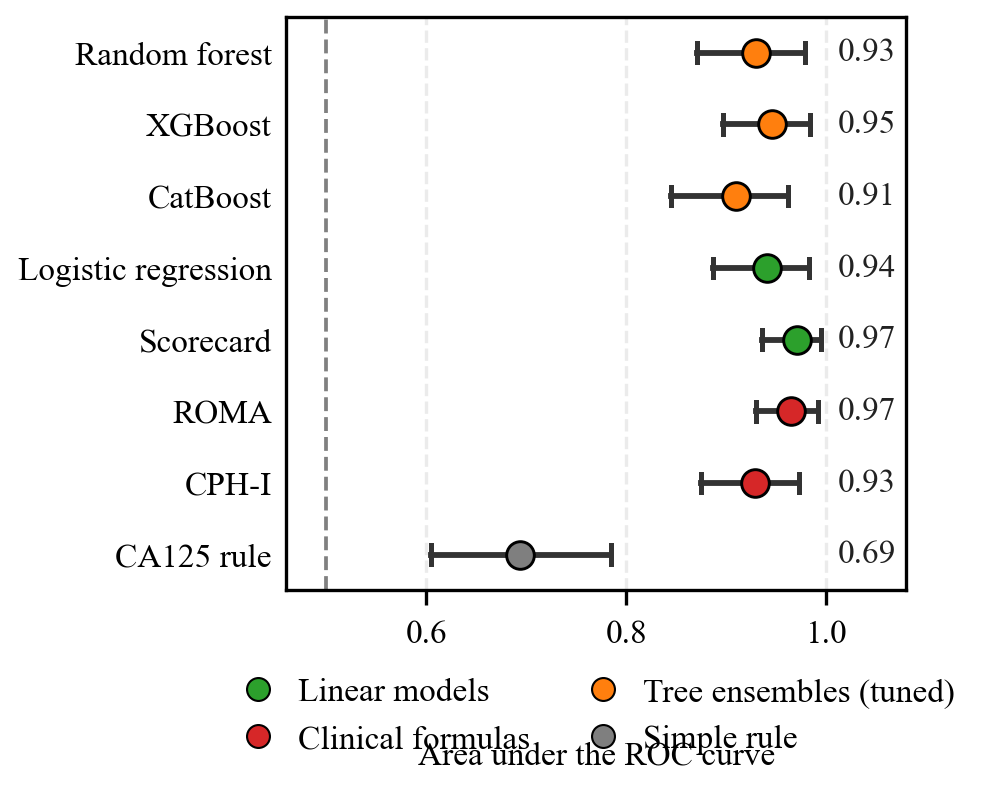
\includegraphics[width=\columnwidth]{figures/fig1_auroc}
\caption{External validation AUROC, 100 West China patients with
measured HE4 (63 cancers). Dots: bootstrap means with 95\% CIs (2{,}000
resamples).}
\label{fig:ladder}
\end{figure}

\subsection{Decision consequences}
\label{sec:results}

In the primary weighted-harm analysis (Q2; Table~\ref{tab:harm},
Figure~\ref{fig:cons}), every model was within-cohort recalibrated. The scorecard's minimum harm was below
recalibrated ROMA and CPH-I at weights up to 5 (12.1
vs.\ 14.7 and 15.0 at $w=1$); at $w=50$, both recalibrated formulas
fell below it (ROMA 45.8, CPH-I 50.3, vs.\ 59.5). The
logistic regression was lowest up to $w=10$; at $w=50$,
recalibrated ROMA was lowest (45.8). Reported minima are over the swept
thresholds; where a minimum exceeds treat-all (e.g., XGBoost at
$w=50$), treating everyone dominates (Table~\ref{tab:harm}).

\begin{figure}[!t]
\centering
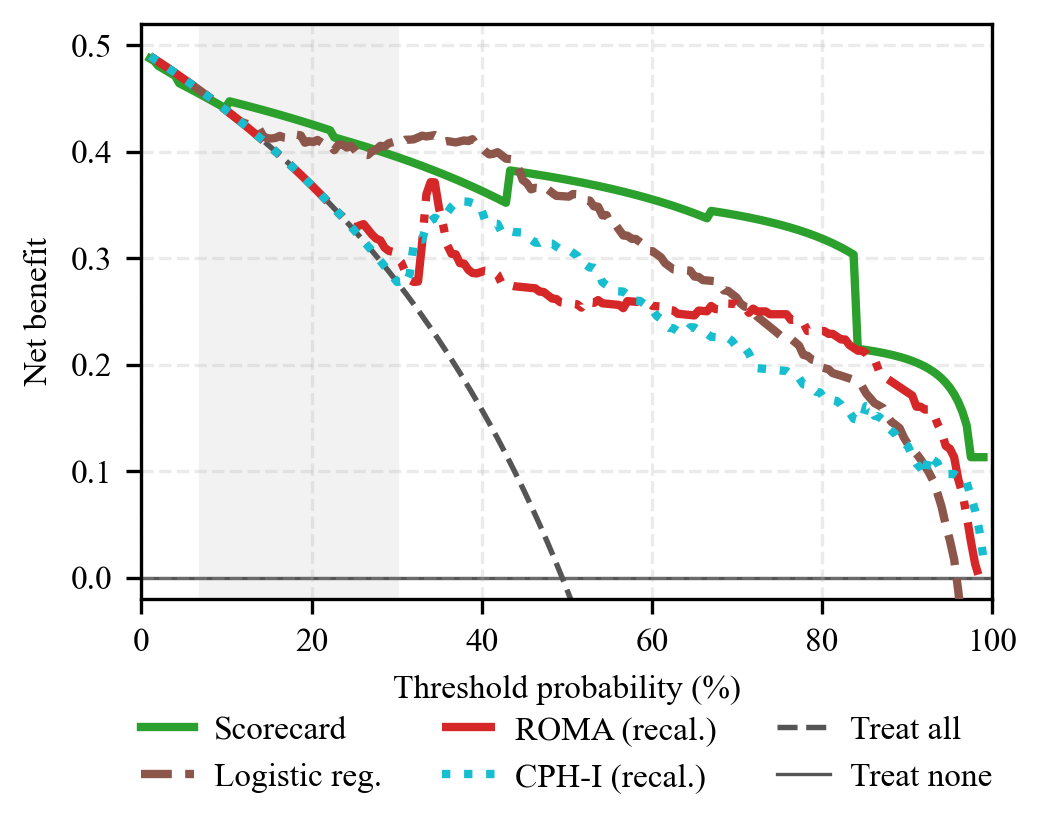
\includegraphics[width=\columnwidth]{figures/fig2_cons}
\caption{Decision curve analysis on West China (N~$=$~380): net benefit
per patient (true positives minus threshold-weighted false positives)
against the decision threshold in percent,
with treat-all (dashed) and treat-none (the horizontal axis)
references; the shaded band marks the published-cutpoint range
(7--30\%). The
scorecard and the two formulas are shown after within-cohort
recalibration. XGBoost is omitted; minimum harms are in
Table~\ref{tab:harm}.}
\label{fig:cons}
\end{figure}

\begin{table}[!t]
\caption{Minimum net harm on West China ($N=380$) at exchange-rate
weight $w$: harm $=w\times$missed$+$unnecessary per 100 women,
minimized over the swept thresholds; treating everyone costs 50.5 at
every weight. Lower is better. Q2 rows: scorecard,
ROMA, and CPH-I are within-cohort recalibrated; the logistic regression
and XGBoost are shown as fitted. Q1 published-scale harms: ROMA
15.0/43.4/45.8/45.8; CPH-I 15.0/51.3/64.7/159.5.}
\label{tab:harm}
\centering
\begin{tabular}{lcccc}
\toprule
Model & $w{=}1$ & $w{=}5$ & $w{=}10$ & $w{=}50$\\
\midrule
Logistic reg. & \textbf{9.7} & \textbf{29.2} & \textbf{39.7} & 46.6\\
Scorecard & 12.1 & 30.5 & 45.0 & 59.5\\
ROMA (recalibrated) & 14.7 & 42.9 & 45.8 & \textbf{45.8}\\
CPH-I (recalibrated) & 15.0 & 50.3 & 50.3 & 50.3\\
XGBoost & 14.7 & 44.7 & 66.1 & 215.5\\
Treat all (reference) & 50.5 & 50.5 & 50.5 & 50.5\\
\bottomrule
\end{tabular}
\end{table}

As the Q1 decision consequence (unchanged transport), the
scorecard's high-risk tier (score $\ge +1$) missed 47 of 188 cancers
with 5 false positives, versus 82 (ROMA) and 48 (CPH-I) at the
published cutpoints.

\subsection{Calibration and missing-data checks}
\label{sec:calibration}

For calibration on the imputed cohort, the
scorecard's logistic mapping was refit on West
China; the logistic regression is shown frozen from training, and the
formulas at published scales. Because the scorecard's fitting and
evaluation share the cohort, these are apparent-calibration
figures, not prospective ones, and only its figures can be inflated by
the shared data.
The recalibrated scorecard had Brier 0.097, a probability-scale
calibration slope of 1.00, and expected calibration error (ECE) of
0.042; the logistic regression had Brier 0.111, slope 1.44, and ECE
0.135. The published
formulas were farther from the data: ROMA had Brier 0.209, slope 1.53,
and ECE 0.220; CPH-I had Brier 0.259, slope 1.11, and ECE 0.303. Both
over-predicted risk (calibration-in-the-large $-0.95$ and $-1.42$).

Refitting without HE4 gave 0.925 (scorecard), 0.932 (logistic
regression), and 0.891 (XGBoost).
Multiple imputation by chained equations (MICE) preserved the
flexible-model ranking (logistic regression 0.926) but degraded the
scorecard's tertile binning (0.853).

\subsection{Robustness and simulation}

Under 30\% multiplicative noise (West China, $N=380$), losses were
0.040 for the scorecard, 0.002 for the logistic regression, 0.074 for
ROMA, and 0.086 for XGBoost.

In the simulation (Figure~\ref{fig:regime}), the
ensemble-average minus-scorecard gap averaged $+0.018$ at drift level
$d=0$ of \eqref{eq:eta} and $-0.018$ at $d=1$; at $d=1$ the scorecard had the
highest AUROC in 22 of 24 cells. Across the four simulation
factors, the spread of the gap was largest across drift levels (0.033), followed by
distribution shift (0.012), training size (0.003), and noise (0.002).

\begin{figure*}[!t]
\centering
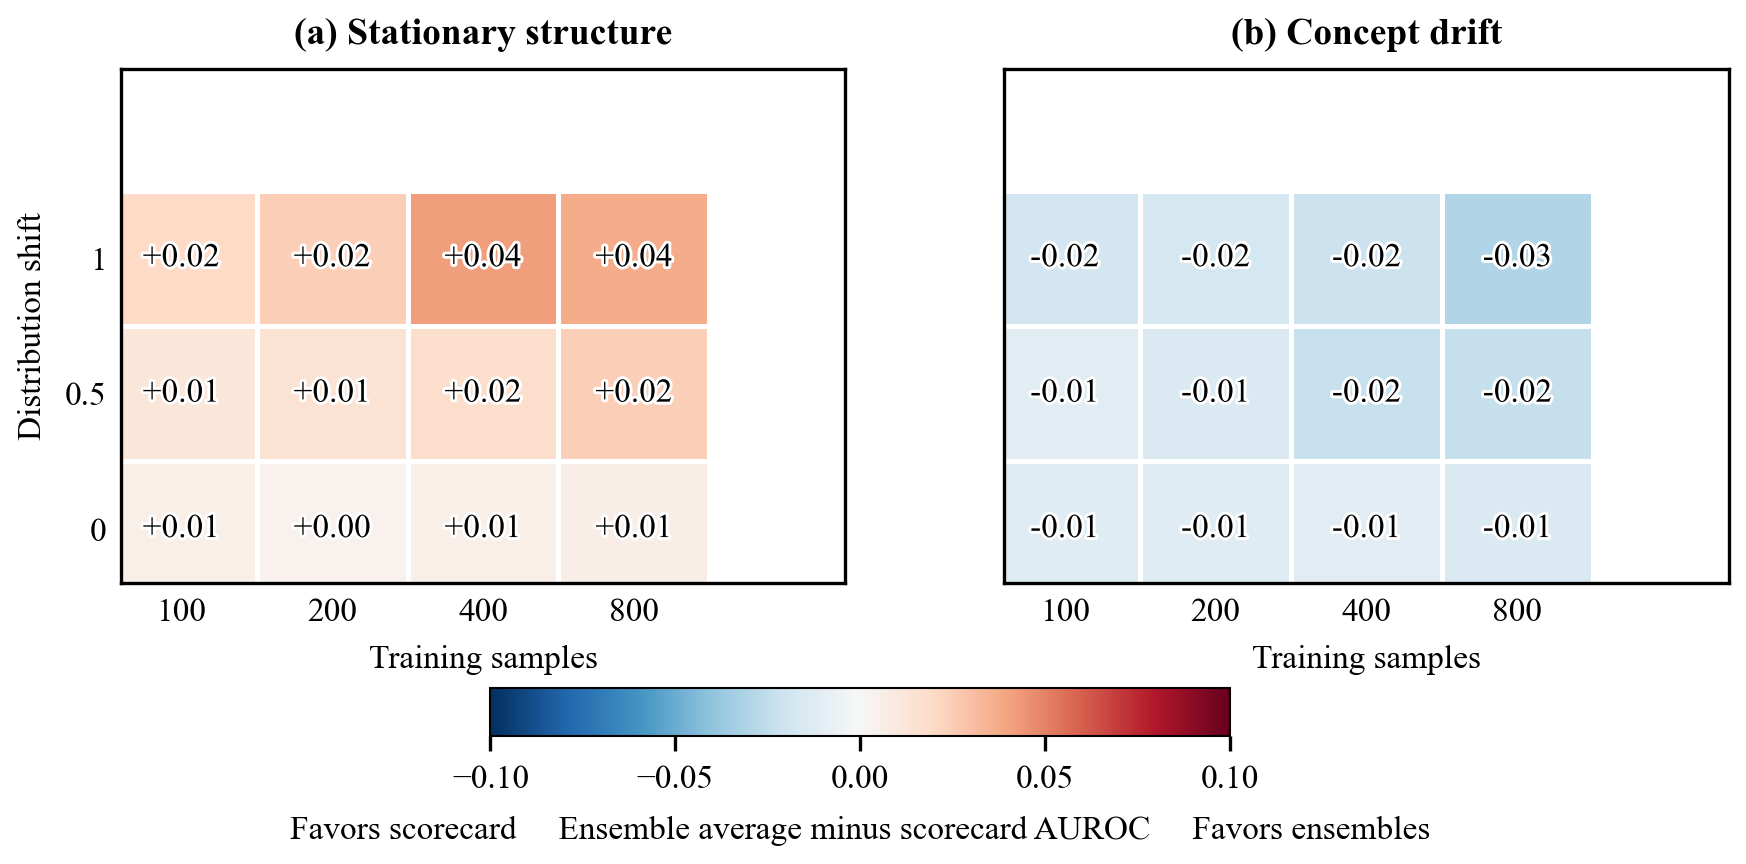
\includegraphics[width=\textwidth]{figures/fig3_regime_col}
\caption{Regime map from the simulation: each cell is the mean over 20
replicates of the ensemble-average minus scorecard test AUROC at
50\% noise; red favors the ensembles, blue the scorecard.
Axes: training samples $n\in\{100,200,400,800\}$; distribution shift
$s\in\{0,0.5,1.0\}$.}
\label{fig:regime}
\end{figure*}

\subsection{Internal validity and sensitivity}
\label{sec:internal}

Across 20 repeated five-fold cross-validations, the scorecard's internal
AUROC was 0.906 (SD 0.003), and the deployed three-bin configuration was
selected in 18 of 20 repeats. In-sample the ensembles fitted at
0.991--1.000, falling 0.094--0.117 under CV. 

\section{Discussion and Conclusion}

The results show three things. First, on discrimination: greater model
complexity did not consistently yield better external performance;
seven integer parameters were not distinguishable from models
with thousands of parameters---the scorecard was
numerically best on the complete cases (0.971), the logistic regression
was highest on the imputed cohort (0.936 vs.\
0.929), and CPH-I won the Japan stress test (0.920). Second, on
decisions: the published cutpoints missed 82 of 188 cancers versus 47
for the scorecard's fixed high-risk tier, and with all models
recalibrated its minimum harm stayed lowest up to 5:1. Third, on
transportability: the simulation offers one possible explanation---
flexible models can exploit interaction and
nonlinear patterns that do not persist; when those
patterns were removed, the scorecard had the highest AUROC in 22 of 24
cells.

The main limitations are as follows. (i) All three cohorts are Asian
hospital series, so results may not transfer to other populations. (ii) HE4 was missing for 74\% of West China
patients and age for 85\% of Japan patients, so much of the external
comparison rests on training-set constants; and the Japanese cohort
consists of healthy volunteers rather than women with masses, so its
discrimination is not directly comparable with West China's; both
narrow how broadly the findings apply. (iii) ultrasound-based models could not be tested (the public
data lack imaging); (iv) the simulation is a simplification, not a
proof about any specific hospital.

Future work should add ultrasound variables and validate
prospectively in larger, multi-center cohorts; on these small cohorts
the scorecard already performed no worse than far more complex models
and stayed fully transparent.

\section*{Acknowledgment}
The authors acknowledge the use of Google Gemini, an AI-based
assistant, for grammar and language checks and for basic code
debugging; the authors retain full authority and responsibility for
the design, methodology, analysis, and all claims of this paper.

\begin{thebibliography}{00}
\bibitem{moore2011} R. G. Moore, M. C. Miller, P. Disilvestro, et al.,
``Evaluation of the diagnostic accuracy of the risk of ovarian malignancy
algorithm in women with a pelvic mass,'' \emph{Obstet. Gynecol.}, vol. 118,
no. 2, pp. 280--288, 2011.
\bibitem{karlsen2015} M. A. Karlsen, E. V. S. H{\o}gdall, I. J. Christensen,
et al., ``A novel diagnostic index combining HE4, CA125 and age may improve
triage of women with suspected ovarian cancer,'' \emph{Gynecol. Oncol.},
vol. 138, no. 3, pp. 640--646, 2015.
\bibitem{kawakami2019} E. Kawakami, J. Tabata, N. Yanaihara, et al.,
``Application of artificial intelligence for preoperative diagnostic and
prognostic prediction in epithelial ovarian cancer based on blood
biomarkers,'' \emph{Clin. Cancer Res.}, vol. 25, no. 10, pp. 3006--3015,
2019.
\bibitem{christodoulou2019} E. Christodoulou, J. Ma, G. S. Collins,
E. W. Steyerberg, J. Y. Verbakel, and B. Van Calster, ``A systematic review
shows no performance benefit of machine learning over logistic regression
for clinical prediction models,'' \emph{J. Clin. Epidemiol.}, vol. 110,
pp. 12--22, 2019.
\bibitem{wynants2020} L. Wynants, B. Van Calster, G. S. Collins, et al.,
``Prediction models for diagnosis and prognosis of COVID-19: systematic
review and critical appraisal,'' \emph{BMJ}, vol. 369, p. m1328, 2020.
\bibitem{lu2020} M. Lu, Z. Fan, B. Xu, et al., ``Using machine learning
to predict ovarian cancer,'' \emph{Int. J. Med. Inform.}, vol. 141,
p. 104195, 2020.
\bibitem{rudin2019} C. Rudin, ``Stop explaining black box machine learning
models for high stakes decisions and use interpretable models instead,''
\emph{Nat. Mach. Intell.}, vol. 1, no. 5, pp. 206--215, 2019.
\bibitem{caruana2015} R. Caruana, Y. Lou, J. Gehrke, P. Koch, M. Sturm,
and N. Elhadad, ``Intelligible models for healthcare: predicting pneumonia
risk and hospital 30-day readmission,'' in \emph{Proc. 21st ACM SIGKDD},
2015, pp. 1721--1730.
\bibitem{ustun2016} B. Ustun and C. Rudin, ``Supersparse linear integer
models for optimized medical scoring systems,'' \emph{Mach. Learn.},
vol. 102, no. 3, pp. 349--391, 2016.
\bibitem{dataset1} Q. Mi, J. Jiang, T. Znati, et al., ``Data for: Using
machine learning to predict ovarian cancer,'' Mendeley Data, vol. 11,
2020, doi: 10.17632/th7fztbrv9.11.
\bibitem{dataset2} Li, ``Comparative analysis of clinical characteristics
between ovarian cancer and ovarian cyst patients,'' figshare, 2025,
doi: 10.6084/m9.figshare.28831256.
\bibitem{machida2023} H. Machida, T. Hirakawa, K. Tsunekawa,
T. Kimura, M. Murakami, and Y. Abe, ``Revised cut-off value of human
epididymis protein 4 enhances its use as an ovarian tumor marker,''
\emph{Gynecol. Obstet. Invest.}, vol. 88, no. 6, pp. 349--358, 2023.
\bibitem{rolfsen2020} A. L. D. Rolfsen, A. A. Dahl, A. H. Pripp, and
A. D{\o}rum, ``Base rate of ovarian cancer on algorithms in patients with
a pelvic mass,'' \emph{Int. J. Gynecol. Cancer}, vol. 30, no. 11, pp.
1775--1779, 2020.
\bibitem{chen2016} T. Chen and C. Guestrin, ``XGBoost: a scalable tree
boosting system,'' in \emph{Proc. 22nd ACM SIGKDD}, 2016, pp. 785--794.
\bibitem{prokhorenkova2018} L. Prokhorenkova, G. Gusev, A. Vorobev,
A. V. Dorogush, and A. Gulin, ``CatBoost: unbiased boosting with
categorical features,'' in \emph{Adv. Neural Inf. Process. Syst.},
vol. 31, 2018.
\bibitem{breiman2001} L. Breiman, ``Random forests,'' \emph{Mach. Learn.},
vol. 45, no. 1, pp. 5--32, 2001.
\bibitem{dersimonian1986} R. DerSimonian and N. Laird, ``Meta-analysis in
clinical trials,'' \emph{Control. Clin. Trials}, vol. 7, no. 3, pp.
177--188, 1986.
\bibitem{vancalster2019} B. Van Calster, D. J. McLernon, M. van Smeden,
L. Wynants, and E. W. Steyerberg, ``Calibration: the Achilles heel of
predictive analytics,'' \emph{BMC Med.}, vol. 17, p. 230, 2019.
\bibitem{vickers2006} A. J. Vickers and E. B. Elkin, ``Decision curve
analysis: a novel method for evaluating prediction models,'' \emph{Med.
Decis. Making}, vol. 26, no. 6, pp. 565--574, 2006.
\bibitem{roberts2021} M. Roberts, D. Driggs, M. Thorpe, et al., ``Common
pitfalls and recommendations for using machine learning to detect and
prognosticate for COVID-19 using chest radiographs and CT scans,''
\emph{Nat. Mach. Intell.}, vol. 3, no. 3, pp. 199--217, 2021.
\end{thebibliography}

\section*{Appendix A. Glossary of Terms}
AUROC: area under the ROC curve; CA125: cancer antigen 125; HE4:
human epididymis protein 4.

\end{document}
